\documentclass[
  digital, %% This option enables the default options for the
           %% digital version of a document. Replace with `printed`
           %% to enable the default options for the printed version
           %% of a document.
  oneside, %% This option enables double-sided typesetting. Use at
           %% least 120 g/m² paper to prevent show-through. Replace
           %% with `oneside` to use one-sided typesetting; use only
           %% if you don’t have access to a double-sided printer,
           %% or if one-sided typesetting is a formal requirement
           %% at your faculty.
  notable,   %% This option causes the coloring of tables. Replace
           %% with `notable` to restore plain LaTeX tables.
  lof,     %% This option prints the List of Figures. Replace with
           %% `nolof` to hide the List of Figures.
  lot,     %% This option prints the List of Tables. Replace with
           %% `nolot` to hide the List of Tables.
  %% More options are listed in the user guide at
  %% <http://mirrors.ctan.org/macros/latex/contrib/fithesis/guide/mu/econ.pdf>.
]{fithesis3}
%% The following section sets up the locales used in the thesis.
\usepackage[resetfonts]{cmap} %% We need to load the T2A font encoding
\usepackage[utf8]{inputenc}
\usepackage[T1]{fontenc}  %% to use the Cyrillic fonts with Russian texts.
\usepackage[
  main=slovak, %% By using `czech` or `slovak` as the main locale
                %% instead of `english`, you can typeset the thesis
                %% in either Czech or Slovak, respectively.
  english, german, russian, slovak %% The additional keys allow
]{babel}        %% foreign texts to be typeset as follows:
%%
%%   \begin{otherlanguage}{german}  ... \end{otherlanguage}
%%   \begin{otherlanguage}{russian} ... \end{otherlanguage}
%%   \begin{otherlanguage}{czech}   ... \end{otherlanguage}
%%   \begin{otherlanguage}{slovak}  ... \end{otherlanguage}
%%
%% For non-Latin scripts, it may be necessary to load additional
%% fonts:
\usepackage{paratype}



%%
%% The following section sets up the metadata of the thesis.
\thesissetup{
    date               = \the\year/\the\month/\the\day,
    autoLayout         = false,
    university         = mu,
    faculty            = econ,
    type               = bc,
    field              = Hospodárska politika,
    department         = Katedra ekonómie,
    author             = Lenka Štefanidesová,
    gender             = f,
    advisor            = {Ing. Rostislav Staněk, Phd.},
    extra              = {
      advisorSkGenitiv = {Ing. Rostislava Staňeka, Phd.}
    },
    title              = { \makecell[l]{Motivačný efekt priebežného výsledku: \\ Robustnosť evidencie zo športových zápasov}},
    TeXtitle           = Motivačný efekt priebežného výsledku: Robustnosť evidencie zo športových zápasov,
    keywords           = {keyword1, keyword2, ...},
    TeXkeywords        = {keyword1, keyword2, \ldots},
    abstract           = {This is the abstract of my thesis, which
                          can

                          span multiple paragraphs.},
    thanks             = {These are the acknowledgements for my
                          thesis, which can

                          span multiple paragraphs.},
    bib                = bibliografia.bib,
    %% Uncomment the following line (by removing the % symbol at
    %% the beginning) and replace `assignment.pdf` with the
    %% filename of your scanned thesis assignment.
    % assignment    = assignment.pdf,
    %% The following keys are only useful, when you're using a
    %% locale other than English. You can safely omit them in an
    %% English thesis.
    titleEn            = { \makecell[l]{Incentive effect of intermediate result: \\ Robustness check of sport matches evidence}},
    TeXtitleEn         = Incentive effect of intermediate result: Robustness check of sport matches evidence,
    keywordsEn         = {keyword1, keyword2, ...},
    TeXkeywordsEn      = {keyword1, keyword2, \ldots},
    abstractEn         = {This is the English abstract of my
                          thesis, which can

                          span multiple paragraphs.},
}
\usepackage{makeidx}      %% The `makeidx` package contains
\makeindex                %% helper commands for index typesetting.
%% These additional packages are used within the document:
\usepackage{paralist} %% Compact list environments
\usepackage{amsmath}  %% Mathematics
\usepackage{amsthm}
\usepackage{amsfonts}
\usepackage{url}      %% Hyperlinks
\usepackage{markdown} %% Lightweight markup
\usepackage{listings} %% Source code highlighting
\lstset{
  basicstyle      = \ttfamily,%
  identifierstyle = \color{black},%
  keywordstyle    = \color{blue},%
  keywordstyle    = {[2]\color{cyan}},%
  keywordstyle    = {[3]\color{olive}},%
  stringstyle     = \color{teal},%
  commentstyle    = \itshape\color{magenta}}
\usepackage{floatrow} %% Putting captions above tables
\floatsetup[table]{capposition=top}
\floatsetup[figure]{capposition=top}
\usepackage{chngcntr}
\counterwithout{table}{chapter}  % Flat numbering of tables.
\counterwithout{figure}{chapter} % Flat numbering of figures.


\usepackage{makecell}
\usepackage{multirow}
\usepackage{hyperref}
\usepackage[noabbrev,capitalise]{cleveref}
\usepackage{textcomp}

\begin{document}
	\makeatletter
	\thesis@preamble %% Print the preamble.
	\makeatother
	
	\chapter*{Úvod}
	\addcontentsline{toc}{chapter}{Úvod}
	
	V bakalárskej práci „Motivačný efekt priebežného výsledku: Robustnosť evidencie zo športových zápasov“ sa zameriavame na skúmanie športových dát, ktoré predstavujú vhodné laboratórium pre štúdium motivačných efektov.
	
	Naša práca primárne vychádza zo štúdie Bergera a Popa (2011), ktorí na základe dát z NBA ukazujú, že tesná prehra v priebehu hry, špecificky v polčase, má silný motivačný efekt. 
	
	V rámci našej práce hľadáme odpovede na otázky \textit{Sú výsledky Berger a Popa robustné? Funguje motivačný efekt rovnako pre mužov ako aj pre ženy? Je rozdiel vo výsledkoch medzi favoritmi a tými ostatnými?} Cieľom našej práce je na dátach z viac ako dvadsať jedna tisíc basketbalových zápasov a piatich rôznych líg overiť robustnosť tohto ich záveru. Okrem toho máme za cieľ preskúmať ako sa líši efekt priebežného výsledku medzi pohlaviami, tj. či existuje ako pri mužoch tak aj pri ženách, po prípade na ktoré pohlavie vplýva silnejšie. Naše očakávanie je, že efekt by mal byť zhruba rovnaký pri mužoch aj pri ženách. Posledným dielčim cieľom tejto práce je porovnať vplyv motivačného efektu pre skupinu favoritov a skupinu tých druhých, nie silne favorizovaných. Dôvodom pre toto skúmanie je overenie nášho predpokladu, že motivačný efekt bude ťahaný práve favoritmi.
	
	\textbf{Prvá kapitola je krátkym úvodom do problematiky...}
	
	\textbf{Druhá kapitola už uvádza čitateľa priamo do problematiky fiškálnych inštitúcií. Vymedzuje tento pojem prostredníctvom jeho štyroch komponentov (fiškálne pravidlá, pravidlá pre zostavovanie rozpočtu, pravidlá transparentnosti, nezávislé inštitúcie) a uvádza nielen tri úrovne fiškálnych inštitúcii ale aj pravidlá, ktorými sú tvorené, limity, ktoré sa ich týkajú, prípadné sankcie, ktoré ich môžu postihnúť a organizácie, ktoré majú nad nimi dozor}.
	
	V poradí tretia kapitola je literárnym rešeršom teórie motivačného efektu. Okrem štúdie Bergera a Popa obsahuje ďalšie 4 práce, ktoré sa venujú tejto tematike. Kapitola sa zameriava vecné zhrnutie stanovených cieľov, zvolených metód riešenia, využitých nástrojov a dosiahnutých výsledkov. 
	
	Štvrtá kapitola je krátkym úvodom do problematiky basketbalu ako športu, v rámci ktorej sú v stručnosti popísané základné pravidlá basketbalu a následne je charakterizovaných päť basketbalových líg, ktorých dáta sú v práci využité.
	
	Piata kapitola začína popisom hlavnej metódy spracovania dát, regresnú diskontinuitu. Ďalej špecifikuje dataset s ktorým sa v práci pracuje, tzn. koľko a akých zápasov obsahuje, aký bol postup spracovania a prispôsobenia dát. Tretia časť kapitoly definuje použitý ekonometrický model a jeho vysvetľovanú a vysvetľované premenné.
	
	Posledná kapitola, šiesta, obsahuje spracovanie dát a popis získaných výsledkov. V závere sú zhrnuté získané poznatky a zodpovedané nastolené otázky z úvodu práce.
	

	\chapter{Prepojenie športu a ekonómie}
	Táto kapitola je krátkym pojednaním o spôsobe, akým sú prepojené dve, na prvý pohľad nijako nesúvisiace, oblasti, akými sú šport a ekonómia.
	
	Šport ako taký, či už na profesionálnej alebo amatérskej úrovni, v súčasnosti zaujal pomerne prominentné miesto v spoločnosti. V podobe zábavného biznisu má celosvetový dosah na milióny ľudí, ktorí sa nielen priamo zúčastňujú najrôznejších zápasov ale čítajú športové články a časopisy či si predplácajú športové televízne stanice a pravidelne sledujú dianie svojho obľúbeného športu. \parencite{conrad2011} Okrem toho sú ľudia denno-denne vyzývaní aby sa sami venovali nejakej športovej aktivite, ktorá je vyzdvihovaná pre svoje zdravotné benefity.
	
	Športová ekonómia je podľa Bootha (\citeyear{booth2009}) kombináciou niekoľkých oblastí ekonomiky, počínajúc napríklad mikroekonomickými princípmi použitými v súvislosti so športovou organizáciou či priemyslom, ekonómiou práce a verejnými financiami. Okrem toho sa športová ekonómia môže zaoberať aj témami rasovej a rodovej diskriminácie alebo reálnym ekonomickým dopadom konania športových udalostí alebo stavby športových zariadení. 
	
	Pre ekonómiu ako vedu je vo všeobecnosti pomerne obtiažne a často krát dokonca nemožné  priamo testovať svoje teórie a hypotézy. Šport sa však vyznačuje jasne zadefinovanými pravidlami a generuje veľké množstvo dát, takže do určitej miery sa dá považovať za ideálne prostredie pre niektoré ekonomické skúmanie a testy.
	
	Práce, ktoré prepájajú ekonómiu a šport sa často krát zameriavajú na profesionálne tímové športy ako basketbal, hokej a americký futbal, keďže tie sú typické práve už spomenutým veľkým objemom najrôznejších kvantitatívnych dát, ktoré pozostávajú nielen z tímových charakteristík, ale aj charakteristík jednotlivcov v rámci súťaže. Ide napríklad o bodovanie, držanie lopty alebo počet odohraných minút v hre.
	
	Autorov zaoberajúcich sa športovou ekonómou je mnoho a ich práce sa líšia nielen poňatím spracovaných tém ale napríklad aj náročnosťou textu. Publikácia od Leedsa (\citeyear{leeds2018}) obsahuje niekoľko konkrétnych príkladov aplikovania mikroekonómie a jej konceptov a teórií priamo na americké a medzinárodné športy, Késenne (\citeyear{kesenne2014}) sa vyznačuje analytickým poňatím teórie profesionálnych tímových športov a autori Sandy, Sloane a Rosentraub (\citeyear{sandy2004}) sa zameriavajú najmä na prípadové štúdie v súvislosti s Spojenými štátmi americkými, Kanadou, Európou a Austráliou. Odlišnou je publikácia Kupera a Syzmanskeho (\citeyear{kuper2009}), ktorá cez ekonómiu, ale aj štatistiku, psychológiu a teóriu hier odpovedá na mnohé zaujímavé otázky týkajúceho sa futbalu, napr. prečo sú krajiny ako Brazília, Nemecko a Španielsko vo futbale úspešné ale Anglicko nie. Foer (\citeyear{foer2004}) zas vo svojej publikácii používa futbal ako prostriedok na vysvetlenie tém ako globalizácia, antisemitizmus či nacionalizmus.
		\section{Teória motivačného efektu}

	\chapter{Literárny rešerš}
	Téma teórie motivačného efektu sa stala predmetom skúmania mnohých autorov. Nasledujúca kapitola obsahuje dovedna 5 prác, ktoré tvoria prehľad literatúry a rôznych prístupov a využitých nástrojov a metód viažucich sa k téme tejto bakalárskej práce, tzn. motivačnému efektu. 
	
		\section{Berger a Pope}
		\label{sec:Berger}
		Hlavnou prácou, o ktorú sa táto bakalárska práca opiera je článok Bergera a Popa (\citeyear{berger2011}) s príznačným názvom \textit{Can Loosing Lead to Winning?} čiže Môže prehrávanie viesť k víťazstvu?. Táto práca ma jednoznačný cieľ a to ukázať na reálnych dátach, že byť trochu pozadu môže v konečnom dôsledku viesť k zvýšeniu šancu na výhru a tak viesť k celkovému víťazstvu a to prostredníctvom ničoho iného ako motivácie.
		
		Rovnako ako táto práca, aj Berger a Pope spracovávali dáta z basketbalových zápasov, skúmali, ako prehrávanie o trochu ovplyvňuje motiváciu a výkon a využili model regresnej diskontinuity. 
		
		Dataset v štúdii tvorilo viac ako 18 000 zápasov profesionálnej NBA, v rozmedzí sezóny 1993/1994 a marca 2009, a viac ako 45 000 zápasov americkej univerzitnej basketbalovej ligy známej pod skratkou NCAA, ktoré sú z obdobia medzi sezónou 1999/2000 a marcom 2009. \parencite[s.~818]{berger2011} Dáta obsahujú okrem informácie kto bol víťazom zápasu aj údaje o bodovom skóre oboch tímov v polčase.
		
		Využitý ekonometrický model mal nasledovnú podobu:
		\begin{equation}
		win_{i} = \alpha + \beta [\textit{losing~at~halftime}]_{i} + \delta [\textit{score~difference~at~halftime}]_{i} + \gamma X_{i} + \varepsilon_{i},
		\end{equation}
		kde \textit{ win $ _{i} $} predstavuje umelú vysvetľovanú premennú, ktorá nadobúda hodnotu jedna keď domáci tím zápas vyhral a nula keď ho prehral, \textit{losing~at~halftime$ _{i} $} je vysvetľujúca premenná, ktorá je taktiež umelou premennou a nadobúda hodnotu jedna keď domáci tím prehráva v polčase o jeden a viac bodov a nula keď vyhráva. Druhou vysvetľujúcou premennou je \textit{score~difference~at~halftime$ _{i} $}, ktorá pozostáva z rozdielu v skóre medzi domácim a hosťujúcim tímom. \textit{Xi} v modeli reprezentuje maticu kontrolných premenných, ktorými sú výherné percentá domáceho a hosťujúceho tímu.  V modeli sa nachádza aj $\alpha$ ako úrovňová konštanta a $\varepsilon_{i}$, čiže náhodná zložka.
		
		Autori v práci menujú niekoľko dôvodov, prečo sa ich pozornosť zameriava práve na polčas. Vyzdvihujú najmä spätnú väzbu v polčase. Vo všeobecnosti spätná väzba pomáha ľuďom upraviť ich postup a snahu tak, aby boli schopní dosiahnuť stanovený cieľ. \parencite{locke2002} V prípade akéhokoľvek športu, nielen basketbalu, je cieľom víťazstvo.
		
		Počas dlhšej pätnásť minútovej prestávky v polčase, oproti stotridsať sekundovej prestávke medzi prvou a druhou a treťou a štvrtou štvrtinou, si tímy a ich jednotliví hráči lepšie uvedomia súčasný stav a bodový rozdiel a tiež to, aké veľké zlepšenie bude potrebné na zníženie súperovho náskoku. Okrem toho je to ideálna príležitosť trénerov zmeniť taktiku hry, prehovoriť hráčom tzv. do duše a vyburcovať ich k lepšiemu výkonu. Keďže je basketbal tímový šport, polčas je vhodným momentom pre utuženie tímového ducha, prediskutovanie prípadných nejasnosti týkajúcich sa spolupráce hráčov a zvýšenie celkovej motivácie.

		
		\renewcommand{\figurename}{Graf}
		\begin{figure}[h]
			\centering
			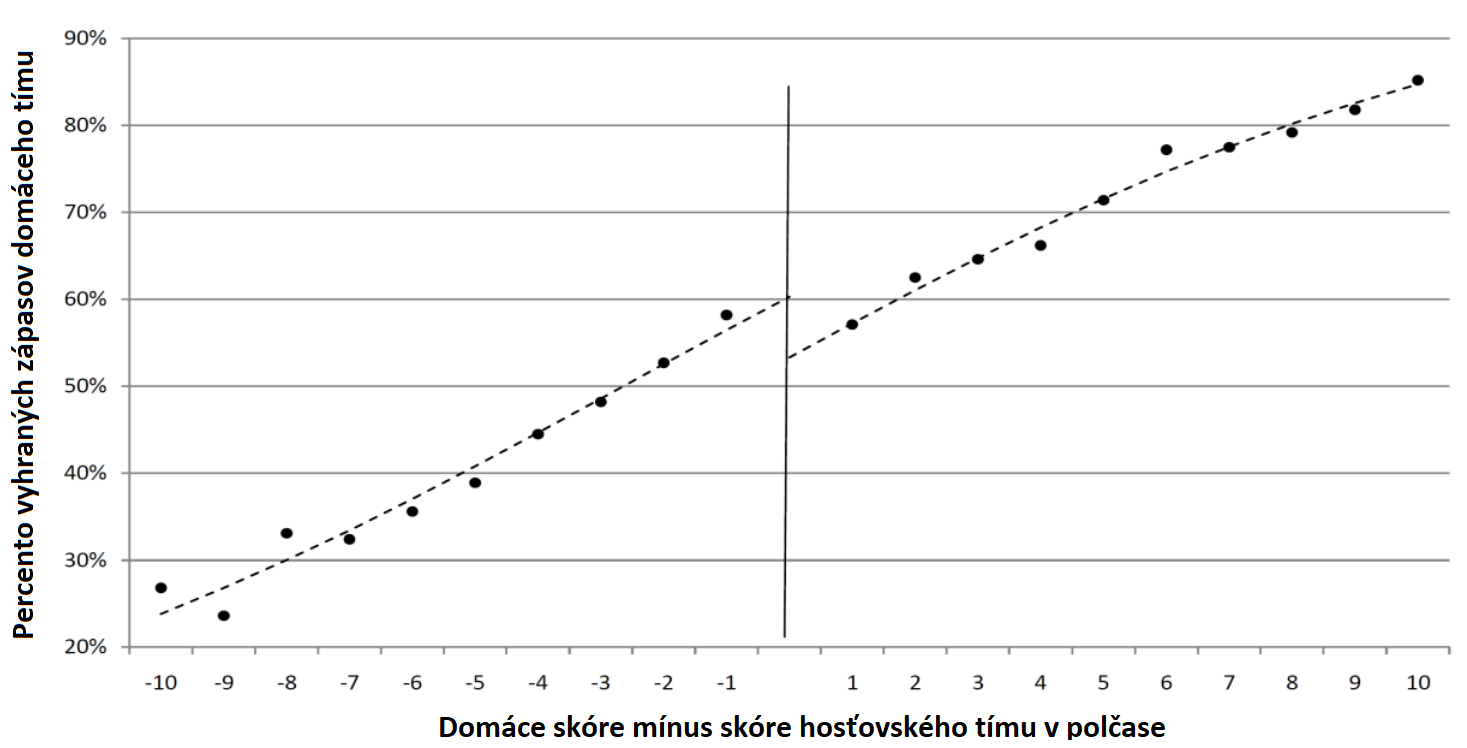
\includegraphics[width=0.8\textwidth]{./grafy/NBA1.png}
			\caption{Percento vyhraných zápasov domáceho tímu na základe bodového rozdielu pre dáta z NBA.}
			\vskip\abovecaptionskip\emph{Zdroj: <<\cite{berger2011} a vlastné spracovanie>>}
			\label{fig:NBA1}
		\end{figure}
	
		Výsledky štúdie v oblasti zápasov NBA potvrdzujú predpoklad autorov z úvodu práce a to, že byť trochu pozadu môže viesť k výhre. Ako vidieť na Grafe \ref{fig:NBA1}, ktorý je vykreslením vzťahu medzi percentom vyhraných zápasov domácim tímom a domácim skóre mínus hosťovským skóre v polčase, že v bode nulového bodového rozdielu existuje diskontinuita. Prerušovaná čiara znázorňuje lineárny tvar dát. 
		
		Ako je vidieť, čím viac tím vyhráva, resp. prehráva v polčase, tým je pravdepodobnejšie, že v konečnom dôsledku vyhrá, resp. prehrá. Avšak výsledky ukazujú aj to, že tímy, ktoré prehrávajú v polčase iba o trochu, vo výsledku vyhrávajú v porovnaní s očakávaním častejšie o 5,8 až 8,0 percentných bodov, viď Tabuľka \ref{table:vplyvNBA1}. Berger a Pope tým hovoria, že namiesto toho, aby domáci tím prehrávajúci o bod mal o približne 5 až 8 percentných bodov nižšiu pravdepodobnosť výhry, takto prehrávajúce tímy sú pravdepodobnejšími víťazmi celého zápasu a vyhrávajú v 58,2\% oproti 57,1\%.
		
		\newcolumntype{x}[1]{>{\centering\hspace{0pt}}p{#1}}
		\newcommand{\sizeofcolumn}{5.4em}
		\begin{table}[t]
			\catcode`\-=12
			\centering 
			\bgroup
			\def\arraystretch{1.5}
			\begin{tabular}{|l||x{\sizeofcolumn}x{\sizeofcolumn}x{\sizeofcolumn}x{\sizeofcolumn}|}
				\hline
				
				\multirow{2}{*}{} & \multicolumn{4}{c|}{Závislá premenná: $ win_{i} $ = 1 ak domáci tím vyhral zápas} \tabularnewline \cline{2-5}
				& (1) & (2) & (3) & (4) \tabularnewline \hline \hline
				
				\multirow{2}{*}{\textit{Prehrávanie v polčase}} & 0,058*** & 0,074*** & 0,062*** & 0,080*** \tabularnewline
				& (0,015) & (0,021) & (0,015) & (0,020) \tabularnewline
				\hline
				
				\textit{Domáci tím} &  &  & 0,0068*** & 0,0068*** \tabularnewline
				\multicolumn{1}{|r||}{\textit{výherné percento}} & & & (0,0002) & (0,002) \tabularnewline
				\hline 
				
				\textit{Hosťujúci tím} &  &  & -0,0065*** & -0,0065*** \tabularnewline
				\multicolumn{1}{|r||}{\textit{výherné percento}} & & & (0,0002) & (0,002) \tabularnewline
				\hline
				
				\textit{Bodový rozdiel v polčase} & X & X & X & X \tabularnewline
				\multicolumn{1}{|r||}{(\textit{lineárny})} & & & & \tabularnewline
				\hline
				
				\textit{Bodový rozdiel v polčase} & & X & & X \tabularnewline
				\multicolumn{1}{|r||}{(\textit{kubický})} & & & & \tabularnewline
				\hline
				
				$ Pseudo-R^{2} $ & 0,097 & 0,097 & 1,172 & 1,172 \tabularnewline
				\hline

				\textit{Pozorovania} & 11 968 & 11 968 & 11 968 & 11 968 \tabularnewline
				\hline
				
			\end{tabular}
			\egroup
			\caption{Vplyv prehrávania v polčase na výhru v NBA dátach}
			\vskip\abovecaptionskip\emph{Zdroj: <<\cite{berger2011} a vlastné spracovanie>>}
			\vskip\abovecaptionskip\emph{Pozn.: V tabuľke sú uvedené hodnoty medzného efektu koeficientov jednotlivých premenných a v zátvorkách je ich smerodatná chyba z použitia logit modelu.}
			\label{table:vplyvNBA1}
		\end{table}	
	
		Okrem NBA ligy skúmali autori aj univerzitnú ligu NCAA a pokúšali sa zistiť, či motivačný efekt bytia pozadu existuje aj v nej. Použitý bol rovnaký typ dát ako aj rovnaké metódy skúmania. Výsledkom je potvrdenie výskytu motivačného efektu aj v tejto vzorke pozorovaní, aj keď sila motivačného efektu v tomto prípade nie je až taká vysoká, čo vidno nielen na Grafe \ref{fig:NCAA} kde je diskontinuita zobrazená menším skokom v bode nulového bodového rozdielu ale aj v Tabuľke \ref{table:vplyvNCAA} v nižších medzných hodnotách koeficientov premennej prehrávania v polčase.
		
		\renewcommand{\figurename}{Graf}
		\begin{figure}[h]
			\centering
			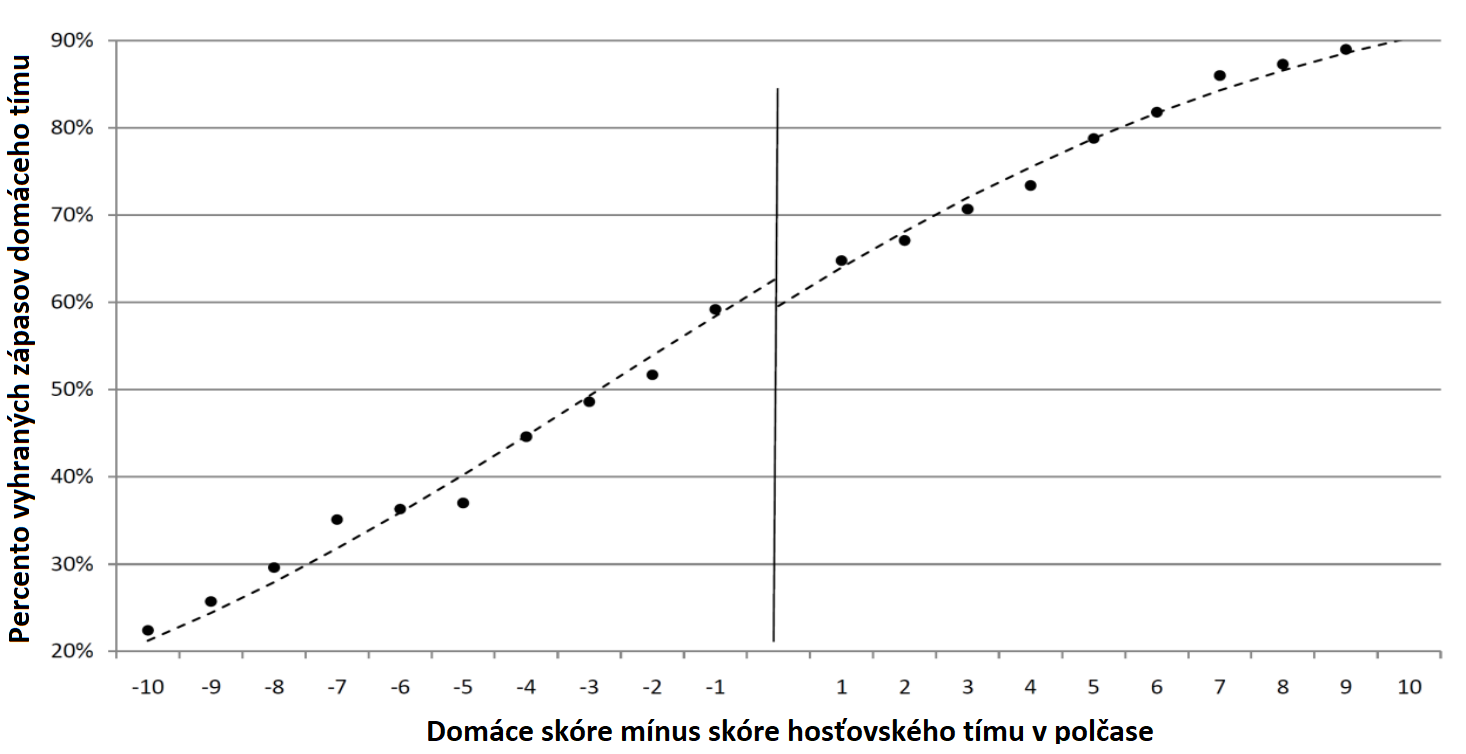
\includegraphics[width=0.8\textwidth]{./grafy/NCAA.png}
			\caption{Percento vyhraných zápasov domáceho tímu na základe bodového rozdielu pre dáta z NCAA.}
			\vskip\abovecaptionskip\emph{Zdroj: <<\cite{berger2011} a vlastné spracovanie>>}
			\label{fig:NCAA}
		\end{figure}
		
		\newcolumntype{x}[1]{>{\centering\hspace{0pt}}p{#1}}
		\begin{table}[t]
			\catcode`\-=12
			\centering 
			\bgroup
			\def\arraystretch{1.5}
			\begin{tabular}{|l||x{\sizeofcolumn}x{\sizeofcolumn}x{\sizeofcolumn}x{\sizeofcolumn}|}
				\hline
				
				\multirow{2}{*}{} & \multicolumn{4}{c|}{Závislá premenná: $ win_{i} $ = 1 ak domáci tím vyhral zápas} \tabularnewline \cline{2-5}
				& (1) & (2) & (3) & (4) \tabularnewline \hline \hline
				
				\multirow{2}{*}{\textit{Prehrávanie v polčase}} & 0,025*** & 0,023* & 0,025*** & 0,021 \tabularnewline
				& (0,010) & (0,014) & (0,009) & (0,013) \tabularnewline
				\hline
				
				\textit{Domáci tím} &  &  & 0,0057*** & 0,0057*** \tabularnewline
				\multicolumn{1}{|r||}{\textit{výherné percento}} & & & (0,0001) & (0,001) \tabularnewline
				\hline 
				
				\textit{Hosťujúci tím} &  &  & -0,0055*** & -0,0055*** \tabularnewline
				\multicolumn{1}{|r||}{\textit{výherné percento}} & & & (0,0001) & (0,0001) \tabularnewline
				\hline
				
				\textit{Bodový rozdiel v polčase} & X & X & X & X \tabularnewline
				\multicolumn{1}{|r||}{(\textit{lineárny})} & & & & \tabularnewline
				\hline
				
				\textit{Bodový rozdiel v polčase} & & X & & X \tabularnewline
				\multicolumn{1}{|r||}{(\textit{kubický})} & & & & \tabularnewline
				\hline
				
				$ Pseudo-R^{2} $ & 0,143 & 0,144 & 0,207 & 0,208 \tabularnewline
				\hline
				
				\textit{Pozorovania} & 29 159 & 29 159 & 28 808 & 28 808 \tabularnewline
				\hline
			\end{tabular}
			\egroup
			\caption{Vplyv prehrávania v polčase na výhru v NCAA dátach}
			\vskip\abovecaptionskip\emph{Zdroj: <<\cite{berger2011} a vlastné spracovanie>>}
			\vskip\abovecaptionskip\emph{Pozn.: V tabuľke sú uvedené hodnoty medzného efektu koeficientov jednotlivých premenných a v zátvorkách je ich smerodatná chyba z použitia logit modelu.}
			\label{table:vplyvNCAA}
		\end{table}	
	
		Po overení a potvrdení predpokladu o fungovaní motivačného efektu bytia pozadu sa autori rozhodli zistiť aj to, kedy má tento efekt najväčší vplyv. Očakávanie autorov bolo, že najväčší vplyv efektu je hneď po polčase, tj. v tretej tretine.
		
		Logit modely vytvorené na overenie tohto predpokladu sa zhodovali s už skôr použitými modelmi až na ten rozdiel, že vysvetľovanou premennou nebola výhra celého zápasu ale v jednom prípade výhra v tretej a v druhom prípade vo štvrtej štvrtine. To znamená, že vysvetľované premenné indikovali to, či mal domáci tím viac bodov na konci danej štvrtiny ako súper. 
		
		Znamienka koeficientov pre premennú prehrávania v polčase sú v oboch prípadoch, pre tretiu aj štvrtú štvrtinu, kladné. Prehrávanie v polčase tým pádom zvýšilo pravdepodobnosť výhry v jednotlivých štvrtinách, avšak väčšie a štatisticky významné sú iba koeficienty pre tretiu tretinu, čím sa predpoklad autorov potvrdil. 			
			
		Vyzdvihnutia hodné je zaujímavé upozornenie autorov, že motivačný efekt polčasového prehrávania je približne polovičnej veľkosti ako všeobecne populárny efekt domácej výhody.

		\section{Merritt a Clauset}
		Basketbal nie je jediný šport, ktorý bol podrobený skúmaniu v súvislosti s teóriou motivačného efektu. Štúdia Merritta a Clauseta (\citeyear{merritt2014}) sa okrem basketbalu venovala aj ďalším športom: americkému futbalu a hokeju. Autori sa zaoberajú pravdepodobnosťou ďalšieho skórovania pri vyhrávaní, resp. prehrávaní a skúmajú, či veľkosť vedenia v zápase poskytuje informáciu o tom, kto získa ďalšie body, tzn. dynamiku skórovania. To samo o sebe nie je predmetom tejto bakalárskej práce, avšak výsledky štúdie \textit{Scoring dynamics across professional team sports: tempo, balance and predictability} obsahujú zaujímavé poznatky aj z oblasti motivačného efektu.
		
		Dataset tejto štúdie je pomerne rozsiahly a predstavujú ho zápasy počas 9 až 10  sezón štyroch amerických športových líg: CFL\footnote{Skratka autorov, ide o Univerzitnú ligu amerického futbalu.}, NFL\footnote{Celý názov National Football League, v preklade Národná futbalová liga.}, NBA a NHL\footnote{Celý názov National Hockey League, v preklade Národná hokejová liga.}. V štúdii autori pracujú s viac ako 40 000 zápasmi, Tabuľka \ref{table:summary1;}, a spracovávajú ich kombináciou Bernoulliho a Poissonovým procesom.
	
		\begin{table}[t]
			\catcode`\-=12
			\centering	
			\bgroup
			\def\arraystretch{1.3}
			\begin{tabular}{|l|c|c|c|c|c|}
				\hline
				\textbf{Šport} & \textbf{Typ} & \textbf{Skratka} & \textbf{Sezóna} & \makecell{\textbf{Počet} \\ \textbf{zápasov}} & \makecell{\textbf{Počet} \\ \textbf{skórovaní}} \\ \hline \hline
				Americký futbal & univerzitný & CFB & 10, 2000-2009 & 14 588 & 120 827 \\
				Americký futbal & pro & NFL & 10, 2000-2009 & 2 654 & 19 476 \\
				Hokej & pro & NHL & 10, 2000-2009 & 11 813 & 44 989 \\
				Basketbal & pro & NBA & 9, 2002-2010 & 11 744 & 1 080 285 \\ \hline				
			\end{tabular}
			\egroup
			\caption{Prehľad dát pre každý šport.}
			\vskip\abovecaptionskip\emph{Zdroj: <<\cite{merritt2014} a vlastné spracovanie>>}
			\label{table:summary1;}
		\end{table}
	
		Výsledky štúdie nie sú totožné naprieč všetkými štyrmi ligami. Pravdepodobnosť ďalšieho skórovania sa v CFL, NFL a NHL zvyšuje s veľkosťou vedenia, zatiaľ čo v prípade NBA, teda basketbalu, sa táto pravdepodobnosť znižuje. Plynutím hry  tak môže dôjsť k zmenšovaniu vedúcej pozície až kým vedenie nezmení v remízu, čo vytvára z basketbalu v podstate nepredvídateľnú hru. Podľa autorov je jedným z možných vysvetlení práve motivačný efekt, kedy sa prehrávajúci tím snaží  jednoducho viac, tzn. že pravdepodobnosť skórovania je vyššia. Nie je však jasné, prečo by sa tento fenomén objavil iba v prípade NBA. \parencite[s.~18]{merritt2014}
	
		Autori však ponúkajú zdôvodnenie, podľa ktorého to môžu spôsobovať stratégie tímov NBA, ktoré sú špecifické práve pre tento šport. Ako príklad je možné spomenúť stiahnutie lepších a skúsenejších hráčov zo zápasu pri vedení, aby sa zbytočne neprepínali  alebo aby sa dokonca nezranili. Bez týchto hráčov sa pravdepodobnosť skórovania pre vedúci tým znižuje. Oproti tomu v hokeji hráči rotujú v jednotlivých formáciách a v americkom futbale sa takéto „náhrady“ nie sú časté. \parencite[s.~19]{merritt2014}
	
		\section{Bergerhoff a Vosen}
		Bergerhoff a Vosen (\citeyear{bergerhoff2015}) sa taktiež zameriavajú na fenomén, kedy byť pozadu, môže byť výhodnejšie. Špecifikom tejto štúdie je testovanie predmetu skúmania prostredníctvom modelovej situácie, tzn. bez použitia reálnych dát.
		
		Výsledné zistenia sú, že cena turnaja, ligy či súťaže, napr. finančné ohodnotenie, trofej alebo prestíž z výhry, a tesná hra motivujú hráčov prekonať prípadnú počiatočnú nevýhodu , vynaložiť viac úsilia a preto majú títo hráči vyššiu pravdepodobnosť výhry. \parencite[s.~20]{bergerhoff2015} Dalo by sa povedať, že keď počiatočné znevýhodnenie silno zvýhodňuje jednu stranu, tá je motivovanejšia a vyvíja väčšiu snahu, avšak keď je rozdiel minimálny a teda tesný, tá strana, ktorá mierne stráca sa ukazuje ako motivovanejšia a snaživejšia.
		
		Tieto výsledky, ako uznávajú aj samotní autori, vysvetľujú a podporujú závery Bergera a Popa (\citeyear{berger2011}), ktoré sú spomenuté vyššie v sekcii \ref{sec:Berger}.
		
		\section{Barankay}
		Rozdielne výsledky priniesla štúdia Barankaya (\citeyear{barankay2010}), ktorá sa síce nezameriava na oblasť športu, avšak skúma do akej miery vie porovnávanie sa s druhými, ktoré prebieha napríklad počas celej dĺžky športových zápasov a ešte viac v čase prestávky, ovplyvniť ľudské správanie a teda zvýšiť alebo znížiť snahu.
		
		Cieľom využitého field experimentu bolo zistiť, ako ľudia prispôsobia svoju snahu v prípade, že dostanú hodnotenie svojej práce v porovnaní s ostatnými zamestnancami. 
		
		Účastníci tohto experimentu, zamestnanci, boli najatí na prácu analýzy obrázkov. Zamestnanci boli následne rozdelení do dvoch skupín, pričom členovia experimentálnej skupiny dostali spätnú väzbu o tom, aké je ich hodnotenie voči ostatným v otázke presnosti ich práce. 
		
		Výsledkom experimentálnej skupiny oproti kontrolnej skupine bola 30\% šanca, že sa zamestnanci do práce nevrátia, a ak sa vrátia, sú o 22\% menej výkonní. To znamená, že závery tejto štúdie poukazujú na fakt, že pri „prehrávaní“ nedochádza k zlepšeniu, práve naopak, prevláda demotivácia. \parencite[s.~4]{barankay2010}
		
		V tomto experimente však hodnotenia nemali vplyv na finančné ohodnotenie zamestnancov, zatiaľ čo pri športových zápasoch by sa dalo argumentovať, že vzájomné porovnávanie dvoch tímov počas zápasu môže ovplyvniť motiváciu tímu iným spôsobom a do inej miery a to za predpokladu, že lepšie výsledky tímu a viac výhier môžu znamenať viac peňazí pre tím a teda lepšie finančné ohodnotenie jednotlivých hráčov.
		
		\section{Schneemann}
		Ďalšou štúdiou, ktorá sa výsledkom nezhoduje s prácou Bergera a Popa (\citeyear{berger2011}) je štúdia Schneemanna a Deutschera (\citeyear{schneemann2017}). Dataset v tomto prípade tvorili zápasy nemeckej futbalovej Bundesligy a to z dvoch sezón  2011/2012 a 2013/2014, čo dovedna tvorí 918 zápasov. Autori na spracovanie dát využívali deskriptívnu štatistiku a regresnú analýzu.
		
		Z mnohých výsledkov a zistení tejto práce sú pre túto bakalársku prácu najrelevantnejšie zistenia týkajúce sa motivácie hráčov počas zápasu v závislosti od jeho vývoja. Pri interpretácií výsledkov je dôležité brať do úvahy bodovanie výsledného skóre futbalového zápasu a medzné straty tímov pri jednotlivých výsledkoch (viď Tabuľka \ref{table:futbal;}).
		
		\begin{table}[t]
			\catcode`\-=12
			\centering	
			\bgroup
			\def\arraystretch{1.2}
			\begin{tabular}{|c|c|c|c|c|}
				\hline
				
				\textbf{Rozdiel v skóre} & \textbf{Stav zápasu} & \textbf{Body} & \textbf{Medzná strata} & \textbf{Medzný zisk} \\ \hline \hline
				$ \leq $ -3 & \multirow{3}{*}{prehra} & 0 & 0 & 0 \\
				-2 &  & 0 & 0 & 0 \\
				-1 &  & 0 & 1 & 0 \\ \hline \hline
				0 & remíza & 1 & 2 & 1 \\ \hline \hline
				1 & \multirow{3}{*}{výhra} & 3 & 0 & 2 \\
				2 &  & 3 & 0 & 0 \\
				$ \geq $ 3 &  & 3 & 0 & 0 \\ \hline				
			\end{tabular}
			\egroup
			\caption{Bodovanie výsledného skóre futbalového zápasu, medzné straty a medzné zisky.}
			\vskip\abovecaptionskip\emph{Zdroj: <<\cite{schneemann2017} a vlastné spracovanie>>}
			\label{table:futbal;}
		\end{table}
		
		Najväčšia motivácia sa prejavila v prípade, keď tím viedol o jeden gól. Akonáhle tím zaostával za súperom o jeden gól, motivácia bola v porovnaní s remízovým skóre alebo vedúcim skóre podstatne nižšia. Autori tento fenomén opodstatňujú hráčskou averziou voči prehre, tzn. že oveľa viac im záleží na tom, aby sa vyhli prehre ako na tom, aby získali výhru. 
		
		V prípade, že tím vedie v zápase jednogólovým rozdielom, stačí jeho súperovi jediný gól na to, aby sa stav zmenil na remízu a doteraz vyhrávajúci tím by prišiel o dva body. Možnosť straty dvoch bodov je pre tím väčším podnetom, ako možnosť získať dva body~\footnote{V situácií remízy.}. 
	
		Rovnaký princíp je uplatniteľný aj o pomyselnú úroveň nižšie, pri porovnávaní remízy a prehrávania o jeden gól, tzn. že tímy sa viac obávajú straty jedného bodu, ktorý by dostali ak by zápas skončil remízou, ako si cenia zisk dodatočného bodu. \parencite[s.~1768]{schneemann2017}
		
		Pravdaže v porovnaní s prácou napr. Bergera a Popa (\citeyear{berger2011}) treba brať do úvahy rozdielnosť povahy skúmaných športov a to najmä v súvislosti s množstvom bodov, ktoré počas jednotlivých zápasov padnú, nakoľko skórovanie v basketbale je, v porovnaní s futbalom, kde často rozhodne jediný gól, oveľa frekventovanejšie.
				
	\chapter{Basketbal ako šport}
	Cieľom tejto kapitoly nie je ísť do podrobností v súvislosti s či už pravidlami alebo históriou jednotlivých líg, ale aspoň v stručnosti definovať basketbal ako šport, keďže naša práca sa týka práve tohto športu, a jednotlivé basketbalové ligy, s ktorých dátami pracujeme.
	
	Basketbal je kolektívny šport desiatich hráčov rozdelených do dvoch súperiacich tímov. Cieľom štyridsaťosem minútovej, resp. štyridsať minútovej hry rozdelenej na štyri štvrtiny je získať viac bodov ako súper. Body sú udeľované za trafenie lopty do basketbalového koša druhého tímu. Počet bodov za jednotlivé skórovania sa líši podľa ich povahy a miesta, z ktorého bol kôš trafený. Kôš hodený z dvojbodového územia je ohodnotený dvomi bodmi, kôš zo vzdialenejšieho územia je za tri body a trestný hod je za jeden bod. Zápasy pritom nemôžu skončiť remízou, podobne ako je to napríklad pri tenise, a v prípade, že sa o víťazovi zápasu nerozhodne v základnej hracej dobe, nastavuje sa toľko päť minútových predĺžení, koľko je potrebné.
	
		\section{Charakteristika basketbalových líg}
		V našej práci budeme pracovať so zápasmi z piatich basketbalových líg a to českou Národnou basketbalovou ligou a Ženskou basketbalovou ligou , americkou Národnou basketbalovou asociáciou a Ženskou národnou basketbalovou asociáciou a Euroligou v basketbale mužov.
		
		Prvé dve ligy sú českými najvyššími basketbalovými ligami. Tou mužskou je Národná basketbalová liga, skrátene NBL, ktorá vznikla v roku 1993 po rozdelení Československa a zániku Československej basketbalovej ligy. Počet basketbalových tímov je dvanásť.
		
		Ženská basketbalová liga, skrátene ŽBL, je najvyššou českou ženskou basketbalovou ligou a 
		vznikla v roku 1993 za rovnakých okolností ako NBL. Súčasný názov však nesie až od roku 2005, premenovaná bola z 1. basketbalovej ligy žien. Počet jej tímov sa v priebehu rokov menil, v súčasnosti je ustálený na rovnakom čísle ako v prípade NBL, takže dvanásť.
		
		Americká Národná basketbalová asociácia, známa pod skratkou NBA, je najpopulárnejšou basketbalovou ligou sveta, ktorá má aj spomedzi tu spomenutých líg najdlhšiu históriu nakoľko vznikla v roku 1946. Delí sa na Východnú a Západnú konferenciu, každá z nich sa ďalej delí na tri divízie, ktoré majú po päť tímov, takže dokopy tvorí NBA tridsať basketbalových klubov.
		
		Ženská národná basketbalová asociácia (WNBA) je ženským náprotivkom mužskej NBA, ktorá sa líši napríklad dĺžkou existencie, počtom tímov či minutážou štvrtín – WNBA bola založená v roku 1994, tvorí ju dvanásť tímov a štvrtiny trvajú desať minút.
		
		Poslednou ligou je tzv. Euroliga, ktorá je európskou basketbalovou mužskou ligou, tvorenou niekoľkými víťazmi národných líg a  niektorými najväčšími európskymi tímami – dokopy ide o šestnásť klubov. 
		
		Každá liga má svoje špecifiká, rozdielov v pravidlách medzi jednotlivými ligami je niekoľko, pre túto prácu však nie sú významné. Spomenúť možno napríklad veľkosť ihriska, vzdialenosť trojbodového skórovania či dĺžku prestávky medzi prvou a druhou a treťou a štvrtou štvrtinou. Okrem toho sa môže líšiť aj systém súťaže. Pre ilustráciu, systém súťaže českej NBL a ŽBL je nasledovný a skladá sa z troch časti: základnej časti, play off a play out. Základná časť, alebo aj tzv. dlhodobá časť, je dvojkolová hra každého tímu s každým – raz doma, raz von. 
		
		Play off sa skladá zo štvrťfinále, semifinále a finále a zápasu o tretie miesto. Štvrťfinále sa hrá na základe umiestnenia tímov v základnej časti podľa vzorca 1-8, 2-7, 3-6, 4-5. Maximálny počet hier vo štvrťfinále je päť, keďže sa hrá na tri víťazné zápasy. Do semifinále teda postupujú štyri najlepšie tímy, ktoré hrajú podľa obdobného vzorca ako vo štvrťfinále, tzn. 1-4 a 2-3 stále na základe umiestnenia zo základnej časti a opäť sa hrá na tri víťazstvá. Následne víťazi zo semifinále postupujú do finále a kto vyhrá zas a opäť ako prvý tri zápasy, získa titul majstra Českej republiky.
		
		Play out je časť súťaže, kedy posledné štyri tímy, teda tie, ktoré sa nedostali do play off, hrajú tzv. kvalifikačnú skupinu formou každý s každým kvalifikačnú skupinu o udržanie sa v NBL. Tím, ktorý sa umiestni na konečnom poslednom mieste zostupuje do nižšej ligy, tj. 1.ligy. Na jeho miesto postúpi práve víťaz 1.ligy, ktorý však môže odmietnuť a v tom prípade je podľa pravidiel táto možnosť postúpená tímu, ktorý skončil na druhom mieste. \parencite{bulletin2018}

	\chapter{Model regresnej diskontinuity a jeho využitie}
		\section{Regresná diskontinuita}
		Použitou metódou v našej práci je tzv. regression discontinuity design, v preklade model regresnej diskontinuity alebo aj nespojitá regresia, známa aj pod skratkou RDD. Ako prví rozpracovali regresnú diskontinuitu autori Thistlethwaite a Campbell (\citeyear{thist1960}), ktorí vo svojej práci skúmali vplyv odmeny za dobré štúdium na budúce akademické úspechy študentov v Spojených štátoch. 
		
		Dobrým štúdiom je myslený dobrý výsledok v teste PSAT~\footnote{Plný angl. názov Preliminary SAT, známy aj ako National Merit Scholarship Qualifying Test.}, ktorý píšu študenti stredných škôl a na základe ktorého sú následne udeľované štipendiá organizáciou NMSC~\footnote{Plný angl. názov National Merit Scholarship Corporation.}. Budúce akademické úspechy predstavuje tzv. GPA~\footnote{Plný angl. názov Grade Point Average je spôsob merania akademickej úspešnosti známy najmä z USA.}.
	
		Skúmanie prebiehalo nasledovne: odmeny vo forme štipendií sú udeľované pri dosiahnutí konkrétneho počtu bodov, tzn. že existuje určitá hranica, ktorá keď je prekonaná, študentovi je udelené štipendium. Naopak, ak študent bodovú hranicu nedosiahne, na štipendium nemá nárok. 
	
		Študenti, ktorí dosiahli bodové ohodnotenie tesne nad a tesne po hranicou sú v podstate rovnakí, alebo aspoň veľmi podobní, avšak tí pod štipendium nezískajú a tí nad áno. Model regresnej diskontinuity porovnáva študentov tesne pod a tesne nad hranicou a rozdiel medzi nimi pripisuje vplyvu udelenia štipendia. 
	
		Očakávania autorov sa v tomto prípade potvrdili. S vyšším počtom získaných bodov  v teste PSAT mali študenti lepšie GPA, avšak vďaka pôsobeniu štipendia sa v hraničnom bode pre zisk štipendia vyskytol nespojitý skok. Tento skok a jeho veľkosť predstavuje odhad RD efektu.
		
		Vo svojej najjednoduchšej podobe má model regresnej diskontinuity následnú podobu:
		
		\begin{equation}
		Y_{i} = \alpha + \beta _{1} [\textit{X}]_{i} + \beta _{2} [\textit{D}]_{i} + \varepsilon_{i}
		\end{equation}
		
		kde 
		
		 \begin{equation}
		D = \begin{cases}
		1 & \text{ak }x\geq{h}, \\
		0 & \text{ak }x < {h}.
		\end{cases}
		\end{equation}
		
		\textit{Y} je vysvetľovaná premenná, $\alpha$ je úrovňová konštanta, premenná \textit{X} je hodnota vysvetľujúcej premennej, \textit{D} je umelá premenná, ktorá vyjadruje či je \textit{X} nad alebo pod hranicou h a $\varepsilon_{i}$ je náhodná zložka. 
		
		To znamená, že pri bližšom pohľade na príklad so štipendiami je hodnota GPA vysvetľovanou premennou \textit{Y}, výsledok v teste PSAT je \textit{X} a \textit{D} nadobúda, napríklad, hodnotu jedna ak je študent nad bodovou hranicou a nula ak je pod ňou.
	
		Ďalším príkladom práce, v ktorej autori využili RDD, je napríklad práca Carpentera a Dobkina (\citeyear{carpenter2011}), ktorí skúmali minimálnu legálnu hranicu pitia alkoholu v USA a jej vplyv na konzumáciu alkoholu mladých ľudí. Banks a Mazzonna (\citeyear{banks2012}) sa zamerali na zvýšenie minimálnej školskej dochádzky zo štrnásť na pätnásť rokov a skúmali vplyv dodatočného roku štúdia na kognitívne schopnosti v staršom veku. Regresnú diskontinuitu má za osvedčenú a efektívnu metódu aj Európska komisia, ktorá ju využíva ako metódu hodnotenia štátnej pomoci. \parencite[s.~20]{ek2014} 
		
		\section{Dataset}
		Využité dáta v tejto práci pochádzajú z databáze športových výsledkov a kurzov Trefík, odkiaľ boli stiahnuté dostupné basketbalové dáta z piatich basketbalových líg – ČBF, ŽBL, NBA, WNBA a Euroligy. \parencite{trefik}
		
		Po stiahnutí dát bolo potrebné ich upravenie a prefiltrovanie na základe predmetu skúmania a potreby nášho modelu, keďže dáta obsahovali či už nadbytočné informácie alebo nemali vhodnú formu. Následné úpravy sa týkali všetkých datasetov, tzn. českého mužského a ženského basketbalu, amerického mužského a ženského basketbalu a európskeho mužského basketbalu.
		
		V prvom rade boli zo všetkých datasetov odstránené tie zápasy, ku ktorým neboli dostupné informácie o bodovom stave v polčase, keďže polčasový stav je pre nami zvolený model kľúčový. Taktiež boli vyradené všetky zápasy ktoré sa skončili remízou, nakoľko v našej práci sa nebudeme zaujímať o výsledky po základnej hracej dobe. Prehľad počtu vyfiltrovaných dát sa nachádza v Tabuľke \ref{table:prefiltrovane-data;}.
		
		Následne boli odstránené nepotrebné dáta relevantných zápasov, ktoré nie sú pre našu prácu potrebné a podstatné, ako napr. dátum zápasu, výsledný bodový stav zápasu či bodový stav za tretiu a štvrtú štvrtinu.
		
		Dáta obsahovali informáciu o víťazovi zápasu, hodnota jedna značila výhru domáceho tímu, hodnota dva jeho prehru, resp. výhru hosťujúceho tímu. Hodnoty dva boli v tomto prípade prekódované na hodnoty nula. Tak nám vznikla premenná \textit{WIN}.
		
		Ďalej bolo potrebné vytvoriť premennú predstavujúcu bodový rozdiel medzi domácim a hosťujúcim tímom v polčase - premennú \textit{SCORE\_HALF}. Vytvoriť preto, lebo takáto informácia nebola priamo dostupná v stiahnutých dátach. Bolo možné ju však odvodiť od  bodového skóre domáceho a hosťujúceho tímu v polčase, ktoré však tiež nebolo priamo v dátach. Na základe bodového stavu po prvej a druhej štvrtine, ktorý dostupný bol, sa však dalo ľahko dopočítať. To znamená, že najprv boli sčítané body za prvú a druhú štvrtinu pre domáci a hosťujúci tím, z čoho vznikli body v polčase pre domáci tím a pre hosťujúci tím. Následne ich rozdielom boli získané dáta pre premennú \textit{SCORE\_HALF}. 
		
		Nutnosťou bolo vytvoriť z dát bodového rozdielu v polčase novú premennú \textit{HALF}, v ktorej bola výhra domáceho tímu po polčase zakódovaná hodnotou nula a prehra hodnotou~jedna. Treba poznamenať, že zápasy, ktoré sa skončili v polčase remízou neboli z datasetu vylúčené, boli v ňom ponechané a kódované ako výhra, nakoľko nás zaujímala zmena šance na výhru, keď sa domáci tím nachádzal striktne pozadu.
		
		Poslednou úpravou dát bolo odčítanie hodnoty jedna od dát predstavujúcich výherný kurz na víťazstvo domáceho tímu.
	
		\begin{table}[t]
			\catcode`\-=12
			\centering	
			\bgroup
			\def\arraystretch{1.3}
			\begin{tabular}{|c|c||c|c|c|c|}
				\hline
					
				\multirow{2}{*}[-1em]{\makecell {\textbf{Basketbalová} \\ \textbf{liga}}}
				& \multirow{2}{*}[-1em]{\textbf{Obdobie}}
				& \multicolumn{4}{c|}{\large\textbf{Zápasy}} \\ \cline{3-6}
									
				& & \makecell{\textbf{Pôvodný} \\ \textbf{počet s dátami}} &  \makecell{\textbf{Remíza} \\ \textbf{v polčase}} & \makecell{\textbf{Remíza} \\ \textbf{na konci}} & \makecell{\textbf{Použitý} \\ \textbf{počet}} \\ \hline \hline
					
				\textit{ČBF} & 2008-2015 & 1 371 & 38 & 46 & 1 325 \\ \hline
				\textit{ŽBL} & 2011-2015 & 556 & 17 & 5 & 551 \\ \hline \hline
					
				\textit{NBA} & 2002-2015 & 15 979 & 569 & 1 009 & 14 970 \\ \hline
				\textit{WNBA} & 2007-2014 & 1 785 & 55 & 135 & 1 650 \\ \hline \hline
					
				\textit{Euroliga} & 2002-2015 & 2 755 & 92 & 128 & 2 627 \\ \hline
			\end{tabular}
			\egroup
			\caption{Prehľad prefiltrovaných dát.}
			\vskip\abovecaptionskip\emph{Zdroj: <<vlastné spracovanie>>}
			\label{table:prefiltrovane-data;}
		\end{table}
	
		Po všetkých vyššie spomenutých úpravách sme mali na ekonometrickú analýzu vhodných dovedna viac ako dvadsať tisíc zápasov. Tabuľka \ref{table:prefiltrovane-data;} poskytuje prehľadný súhrn týchto zápasov, ich príslušnosť k jednotlivým ligám, či rámcové obdobie, z ktorého dané zápasy sú.
		
		Tak ako bolo už niekoľko krát spomenuté, v našej práci porovnávame vždy domáci a hosťujúci tím. Pri každom zápase však skúmame iba jeden z týchto tímov, aby sme sa vyhli duplicite. V zásade je bezpredmetné, či by bol vybraný domáci alebo hosťujúci tím, nakoľko hociktorý jeden je zrkadlovým odrazom toho druhého. Výber v našom prípade je zhodný s výberom Bergera a Popa (\citeyear{berger2011}), ktorí sa rozhodli pre domáci tím. Náhodný výber tímu by nebol v tomto prípade vhodnou metódou, keďže by mohol viesť k rozdielnym výsledkom v závislosti na náhodnosti výberu.
		
		Testovanie následne prebiehalo postupne v rámci jednotlivých líg, čo nám dalo možnosť nielen skúmať rozdiely medzi národnými ligami, ale napríklad aj rozdiely v motivácií v mužských a ženských ligách.
		
		\section{Použitý ekonometrický model}
		Pri zostavovaní ekonometrického modelu sme vychádzali z už spomínanej štúdie Berger and Pope (\citeyear{berger2011}), ktorý bol však pozmenený v súvislosti s našim cieľom práce. Dáta boli spracované vo voľne prístupnom programe Studio R a mali podobu prierezových dát.
		
		Podoba nášho ekonometrického modelu je nasledovná:
		\begin{multline}
		WIN_{i} = \alpha + \beta _{1} [\textit{HALF}]_{i} + \beta _{2} [\textit{SCORE~\_~HALF}]_{i} + \beta _{3} [\textit{SCORE~\_~HALF2}]_{i} \\
		+ \beta _{4} [\textit{SCORE~\_~HALF3}]_{i} + \beta _{5} [\textit{BETTING\_RATE}]_{i} + \varepsilon_{i},
		\end{multline}
		
		Vysvetľovanou premennou je premenná \textit{WIN}, ktorá je umelou premennou nadobúdajúcou hodnotu jedna ak domáci tím vyhrá zápas a nula ak tento zápas prehrá, resp. zápas vyhrá súper. 
		
		Vysvetľujúcich premenných je dovedna päť. Prvou je umelá premenná \textit{HALF}, ktorá nám udáva informáciu o tom, či domáci tím v polčase prehrával alebo vyhrával. Ak vyhrával, premenná nadobúda hodnotu nula a ak prehrával, hodnota je jedna. Zdôvodnením je fakt, že v našej práci nás zaujímajú prípady zápasov, kedy domáci tím v polčase prehrával a predpokladáme, že malá bodová strata na súpera ho motivovala k lepšiemu výkonu a teda zdolaniu súpera a víťazstvu. 
		
		Ďalšou vysvetľujúcou premennou je premenná \textit{SCORE\_HALF}, ktorá udáva bodový rozdiel v polčase medzi dvomi tímami. Premenné \textit{SCORE\_HALF2} a \textit{SCORE\_HALF3} sú umocnením premennej \textit{SCORE\_HALF} na druhú a následne na tretiu. Dôvodom zahrnutia týchto dvoch premenných je, že pravdepodobnosť výhry nemusí byť lineárna v tom, koľko domáci tím prehráva v polčase a s druhým a tretím umocnením premennej \textit{SCORE\_HALF} je možné lepšie prispôsobiť naše dáta tomu, aby bolo možné vidieť skok regresnej diskontinuity,  za predpokladu, že sa tam nachádza.
		
		\textit{BETTING\_RATE} je poslednou vysvetľujúcou premennou, ktorá by mala reprezentovať, ako ovplyvní model to, či je domáci tím favoritom. Iba pre pripomenutie, čím vyššia je premenná, tým vyšší je kurz na víťazstvo domáceho tímu a tím menším favoritom je. Platí teda, že čím nižší kurz, tým je tím väčším favoritom a naopak. Odčítanie hodnoty jedna od kurzu na víťazstvo domáceho tímu nie je nutnosťou, avšak v tejto podobe nám dáva informáciu o čistom zisku z jednotky meny, napr. z jednej koruny a následná interpretácia je relatívne jednoduchšia.
		
		Okrem toho model obsahuje úrovňovú konštantu $\alpha$, parametre vysvetľujúcich premenných $\beta _{1}$ až $\beta _{5}$  a náhodnú zložku $\varepsilon_{i}$.
	
		\begin{table}[t]
			\catcode`\-=12
			\centering	
			\bgroup
			\def\arraystretch{1.3}
			\begin{tabular}{l l}
				\hline
				\textbf{Premenná} & \textbf{Popis} \\ \hline \hline
				\textit{WIN} & výhra, resp. prehra domáceho tímu \\
				\textit{HALF} & výhra, resp. prehra domáceho tímu v polčase \\
				\textit{SCORE\_HALF} &  rozdiel v polčase medzi domácim a hosťujúcim tímom \\
				\textit{SCORE\_HALF2} & rozdiel v polčase umocnený na druhú \\
				\textit{SCORE\_HALF3} & rozdiel v polčase umocnený na tretiu \\
				\textit{BETTING\_RATE} & kurz na víťazstvo domáceho tímu mínus jedna \\ \hline
			\end{tabular}
			\egroup
			\caption{Stručný prehľad vysvetľovanej premennej a vysvetľujúcich premenných.}
			\vskip\abovecaptionskip\emph{Zdroj: <<vlastné spracovanie>>}
			\label{table:premenne;}
		\end{table}

\printbibliography[heading=bibintoc] %% Print the bibliography.
\end{document}